\documentclass{paper}
%\usepackage{nomencl}
\usepackage{nomencl}
\usepackage{amsmath}
\usepackage{graphicx}
\usepackage{subfigure}
\usepackage{parskip}
%\usepackage{minted}
\usepackage[toc,page]{appendix}
\usepackage{csquotes}
\usepackage{framed}
\usepackage{amsthm}

\theoremstyle{theorem}
\newtheorem{theorem}{Theorem}[section]
 
\theoremstyle{definition}
\newtheorem{definition}{Definition}[section]

\theoremstyle{remark}
\newtheorem{remark}{Remark}[section]
%\usepackage{biblatex}
%\makenomenclature
\title{Model Based Engineering}
\author{A. Giavaras}
\date{}

\begin{document}
\maketitle
\tableofcontents


\clearpage


%\section{Output Feedback}
\label{output_feedback}

Chapter \ref{state_feedback} introduced the concept of reachability. It was shown that it is possible to find 
a state feedback law that gives the desired closed loop eigenvalues provided that the system
is reachable.  Furthermore, we saw how to design controllers using
the system state, $x(t)$, as feedback to out controller. 

However, desigining state feedback controllers preassumes that all the states are measured. For many situations, it
is highly unrealistic to assume that all the states are measured. 

In this section we proceed somehow in a similar vein we can use the output $y(t)$ to modify the dynamics of the system through the use of observers. Furthermore, we will introduce the concept of observability
and show that if a system is observable, it is possible to recover the state
from measurements of the inputs and outputs to the system. We then show how to
design a controller with feedback from the observer state. 




\section{Observability}
\label{observability}

For many situations, it is highly unrealistic to assume that all the states are measured. In this section we
investigate how the state can be estimated by using a mathematical model and a
few measurements. It will be shown that computation of the states can be carried
out by a dynamical system called an \textbf{observer}, see also figure \ref{observer_block_diagram}.


\begin{framed}
\theoremstyle{definition}
\begin{definition}{\textbf{Observability}}
A linear system is \textbf{observable}  if for any $T>0$ it is possible to determine the state of the system $x(T)$ through measurements of $y(t)$ and $u(t)$ on the interval $[0,T]$  $x(T) = x_f$.
\end{definition}
\end{framed}


\begin{framed}
\theoremstyle{remark}
\begin{remark}{\textbf{Nonlinear Systems}}

The definition above holds for nonlinear systems as well, and the results discussed here have extensions to the nonlinear case.
\end{remark}
\end{framed}


Consider again the system

\begin{equation}
\frac{dx}{dt} = Ax + Bu ~~ y = Cx + Du
\end{equation}


where $x\in R^n$ is the state, $u\in R^{p}$ is the input and $y\in R^q$ the measured output.

We wish to estimate the state of the system from its inputs and outputs, as illustrated
in Figure \ref{observer_block_diagram}. In some situations we will assume that there is only one measured
signal, i.e., that the signal $y$ is a scalar and that $C$ is a (row) vector. This signal may
be corrupted by noise $n$, although we shall start by considering the noise-free case.
We write $\hat{x}$ for the state estimate given by the observer.

\begin{figure}[!htb]
\begin{center}
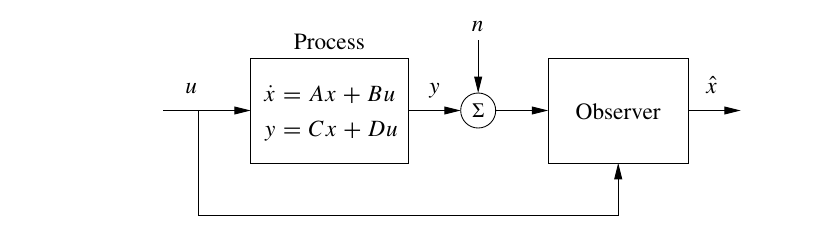
\includegraphics[scale=0.380]{img/output_feedback/observer_block_diagram.jpeg}
\end{center}
\caption{Block diagram for an observer. The observer uses the process measurement $y$
(possibly corrupted by noise $n$) and the input $u$ to estimate the current state of the process,
denoted $\hat{x}$.}
\label{observer_block_diagram}
\end{figure}


The problem of observability is one that has many important applications, even
outside feedback systems. If a system is observable, then there are no hidden dynamics inside it; we can understand everything that is going on through observation (over time) of the inputs and outputs. As we shall see, the problem of observability is of significant practical interest because it will determine if a set of sensors is
sufficient for controlling a system. Sensors combined with a mathematical model
can also be viewed as a virtual sensor that gives information about variables that
are not measured directly. The process of reconciling signals from many sensors
with mathematical models is also called sensor fusion.



\section{Testing for Observability}
\label{test_observability}

When discussing reachability in the last chapter, we neglected the output and focused on the state. Similarly, it is convenient here to initially neglect the input and
focus on the autonomous system



\begin{framed}
\theoremstyle{remark}
\begin{remark}{\textbf{Autonomous System}}

\end{remark}
\end{framed}

\begin{equation}
\frac{dx}{dt} = Ax ~~ y = Cx
\end{equation}

The objective is to understand when it is possible to determine the state from observations of the output. From

\begin{equation}
y = Cx
\end{equation}

we see that the output itself gives us the projection of the state $x$ on vectors that are rows of the matrix $C$. The 
observability problem can  immediately be solved if the matrix $C$ is invertible. If the matrix is not invertible we can take the derivatives and obtain

 
\begin{equation}
\frac{dy}{dt} = C\frac{dx}{dt} = CAx
\end{equation}

From the derivative of the output we thus get the projection of the state on vectors that are rows of the matrix $CA$. Proceeding in this way, we get

\begin{equation}
\begin{bmatrix}
 y \\
 y^{(1)} \\
 \vdots \\
 y^{(n-1)} 
\end{bmatrix} = 
\begin{bmatrix}
 C \\
 CA \\
 \vdots \\
 CA^{n-1} 
\end{bmatrix}x
\end{equation}

We thus find that the state can  be  determined if the observability matrix
 
\begin{equation}
W_o= 
\begin{bmatrix}
 C \\
 CA \\
 \vdots \\
 CA^{n-1} 
\end{bmatrix}
\end{equation}

has $n$ independent rows.  It turns out  that  we  need  not consider any derivatives higher
than $n-1$ (this is an application of the Cayley-Hamilton theorem)
 
\begin{framed}
\theoremstyle{remark}
\begin{remark}{\textbf{System with inputs}}

The calculation can easily be extended to systems with inputs. The state is then
given by a linear combination of inputs and outputs and their higher derivatives.
The observability criterion is unchanged. 
\end{remark}
\end{framed}


\begin{framed}
\theoremstyle{theorem}
\begin{theorem}{\textbf{Observability rank condition}}

A linear system of the form  
\begin{equation}
\frac{dx}{dt} = Ax + Bu, ~~ y = Cx + Du \nonumber
\end{equation}

is observable if and only if the observability matrix $W_o$ is full rank.
\end{theorem}
\end{framed}

\section{Observable Canonical Form}
\label{observability_canonical_form}

As in the case of reachability, certain canonical forms will be useful in studying ob-
servability. A linear single-input, single-output state space system is in observable
canonical form if its dynamics are given by


\begin{framed}
\theoremstyle{remark}
\begin{remark}{\textbf{Observable Canonical Form for Nonlinear Systems}}

The definition can be extended to systems with many inputs; the only difference is
that the vector multiplying u is replaced by a matrix.
\end{remark}
\end{framed}


The characteristic polynomial for a system in observable canonical form is

\begin{equation}
\lambda(s) = s^n +\alpha_1s^{n-1} + \ldots + \alpha_{n-1}s + \alpha_n
\end{equation}

In order to check the observability property of a systme more formally, we can compute the observability matrix for
a system in observable canonical form. This is given by

\begin{equation}
W_o= 
\begin{bmatrix}
 1 & 0 & 0 & \ldots &  0\\
 -\alpha_1 & 1 & 0 & \ldots &  0 \\
 -\alpha_{1}^{2} - \alpha_1 \alpha_2 & - \alpha_1 & 1 &  \ldots &  0 \\
 \vdots & \vdots & \vdots & \ddots & \vdots \\
* & * & * & \ldots & 1
\end{bmatrix} 
\end{equation}


where * represents  an entry  whose exact  value  is  not important.
What is important here is the rows of this matrix are linearly independent (since it is lower triangular), and hence Wo is full rank. Hence, it is invertible. 

As in the case of reachability (see section \ref{reachable_canonical_form}), it  turns  out  that  if a  system  is  observable then there
always exists a transformation $T$ that converts the system into observable canonical
form. This is useful for proofs since it lets us assume that a system is in observable
canonical form without any loss of generality. The observable canonical form may
be poorly conditioned numerically.
 

\section{State Estimation}
State feedback control design, as explained in t chapter \ref{state_feedback} requires that we have access to the complete state vector. 
However, measuring the complete state vector is not always feasible (for example a sensor may not be available at all) and it may also be expensive.
In this section we will introduce the idea of state estimation as a way to get access to the state variables. 


\begin{framed}
\theoremstyle{remark}
\begin{remark}{\textbf{Soft Sensors}}


The concept of using software instead of sensors to access the quantity we are 
interested in, is referred to as soft sensors in the automotive industry.
\end{remark}
\end{framed}

Recall that the idea of state feedback control was to modify the eigenvalues of the system under consideration by using the input

\begin{equation}
u = -Kx + K_r r  
\end{equation}

However, it can be seen that this requires the state vector $x$. The idea of state estimation is to design something called an observer that tries to provide an 
estimate say $\hat{x}$ of the state vector $x$. The observer is fed with the same input as the real plant. The goal of the observer is to provide somehow a replica of the true state vector.
Thus, we would like to have the error $\tilde{x}$ between the two quantities to be zero. Namely,


\begin{equation}
\tilde{x} = x - \hat{x} = 0 
\end{equation}
 
In this section, we want to construct a dynamical system of the form

\begin{equation}
\frac{d \hat{x}}{dt} = F\hat{x} + Gu + Hy  
\end{equation}

where $u$ and $y$ are the input and output of the original system and $\hat{x} \in R^n$ is an estimate of $x$ with the property

\begin{equation}
\hat{x}(t) \rightarrow x(t), ~~ \text{as} ~~ t \rightarrow \infty  
\end{equation}

Let's consider again the system

\begin{equation}
\frac{dx}{dt} = Ax + Bu ~~ y = Cx + Du
\label{sys}
\end{equation}

assume further that $D$ is zero. Assuming that the input $u$ is known, then an estimate of the state $x$ is given by

\begin{equation}
\frac{d\hat{x}}{dt} = A\hat{x} + Bu
\label{observer_one} 
\end{equation}  

We would like to know the properties of this estimate; how far is from the exact state? The estimation error is \cite{Astrom} 

\begin{equation}
\tilde{x} = x - \hat{x} 
\end{equation} 

substituting into equation \ref{observer_one} we find that


\begin{equation}
\frac{d\tilde{x}}{dt} = A\tilde{x}  
\end{equation}  

We already know that the behavior of this system depends on the eigenvalues of $A$. Concretely, if matrix $A$ has all its eigenvalues in the left half-plane, the error $\tilde{x}$ will go to zero,
and hence equation \ref{observer_one} is a dynamical system whose output converges to the state
of the system \ref{sys}.


The observer given by equation \ref{observer_one} uses only the process input $u$; the measured
signal does not appear in the equation. We must also require that the system be stable,
and essentially our estimator converges because the state of both the observer and
the estimator are going zero. This is not very useful in a control design context since
we want to have our estimate converge quickly to a nonzero state so that we can
make use of it in our controller. We will therefore attempt to modify the observer
so that the output is used and its convergence properties can be designed to be fast
relative to the system’s dynamics. This version will also work for unstable systems.

Let's now consider the following observer

\begin{equation}
\frac{d \hat{x}}{dt} = A\hat{x} + Bu + L(y- C \hat{x})
\label{observer_two}   
\end{equation}

The term $L(y- C \hat{x})$ provides feedback and hence the observer in \ref{observer_two} can be seen as a generalization of the observer in \ref{observer_one}. The supplied feedback is proportional to the difference between the observed output and the output predicted by the observer. Substituting the expression for the error $\tilde{x}$ we arraive at

 \begin{equation}
\frac{d\tilde{x}}{dt} = (A-LC)\tilde{x} 
\label{observer_two}   
\end{equation} 

If the matrix $L$ can be chosen in such a way that the matrix $A-LC$ has eigenvalues with negative real parts, the error $\tilde{x}$ will go to zero. The convergence rate is determined by an appropriate selection of the eigenvalues.
 

\begin{framed}
\theoremstyle{remark}
\begin{remark}{\textbf{Observer design and state feedback duality}}


Notice the similarity between the problems of finding a state feedback and
finding the observer. State feedback design by eigenvalue assignment is equivalent
to finding a matrix $K$ so that $A-BK$ has given eigenvalues. Designing an observer
with prescribed eigenvalues is equivalent to finding a matrix $L$ so that $A-LC$ has
given eigenvalues. Since the eigenvalues of a matrix and its transpose are the same
we can establish the following equivalences:

\begin{equation}
A \leftrightarrow A^T, ~~ B \leftrightarrow C^T, ~~ K \leftrightarrow L^T, ~~ W_r \leftrightarrow W_{o}^{T}
\end{equation}

The observer design problem is the dual of the state feedback design problem. 
\end{remark}
\end{framed}



\begin{framed}
\theoremstyle{theorem}
\begin{theorem}{\textbf{Observer design by eigenvalue assignment}}


Consider the system

\begin{equation}
\frac{dx}{dt} = Ax + Bu, ~~ y =Cx   \nonumber
\end{equation} 

with one input and one output. Let the characteristic polynomial related to matrix A be

\begin{equation}
\lambda(s) = s^n + \alpha_1 s^{n-1} + \ldots + \alpha_{n-1}s + \alpha_n \nonumber
\end{equation}

If the systme is observable, then the dynamical system

\begin{equation}
\frac{d \hat{x}}{dt} = A\hat{x} + Bu + L(y- C \hat{x})  \nonumber
\end{equation}


is an observer for the system with $L$ chosen as 

\begin{equation}
L = W_{o}^{-1}\tilde{W}_o
\begin{bmatrix}
 p_1 - \alpha_1 \\
 p_2 - \alpha_2 \\
 \vdots  \\
 p_n - \alpha_n
\end{bmatrix} \nonumber
\end{equation}

The matrices $W_{o}$ and $\tilde{W}_{o}$ are given by

The resulting observer error $\tilde{x}$ is governed by a differential equation that has the following characteristic polynomial

\begin{equation}
p(s) = s^n +  p-1 s^{n-1} + \ldots + p_n  \nonumber
\end{equation}
\end{theorem}
\end{framed}

The dynamical system (7.10) is called an observer for (the states of) the system (7.9) because it will generate an approximation of the states of the system from its inputs and outputs. This form of an observer is a much more useful form than the one given by pure differentiation in equation (7.3).


\section{Questions}

\textbf{Question 1}

What is the main reason for using an estimator in feedback control?

\begin{itemize}
\item A) There are process disturbances in the model 
\item B) We are measuring the wrong quantities 
\item C) It is too expensive or impractical to measure each state variable correct 
\end{itemize} 

\textbf{Answer}  

Option C is the correct answer.


%\section{The Physics of Automotive Dynamics}
\label{physics-automotive_dynamics}
In these notes, we are not particularly interested in how the combustion engine operates. In contrast, we are interested in automobiles as a macroscopic system that we would
like to understand and control. In this context, we will treat the combustion engine (or any other means whatsoever producion the propulsion force) as a black box.
However, we want to be able to argue upon how much force the engine system should produce such that the vehicle is able to accelerate, decelerate or travel at constant speed.
In this chapter therefore, we will introduce the basic physical laws that govern the motion of the vehicle. In particular, we will consider

\begin{itemize}
\item Longitudinal vehicle dynamics
\item Aerodynamic force $\mathbf{F}_{aero}$
\item Rolling force $\mathbf{F}_{roll}$
\item Gravitational force $\mathbf{F}_{grav}$
\end{itemize}

By considering the above mentioned forces, we will be able to produce a basic model that explains the longitudinal dynamics of the vehicle. In chaper \ref{model_automotive_sys} we will get more into modeling the subsystems of the vehicle and come up with a more refined model.


\section{Aerodynamics \& Rolling Resistance}

Let us start simple and assume the motion of a vehicle in a flat road; no road gradietns. There are three types of forces that are always present in such a scenario; the propulsion force, $\mathbf{F}_{p}$, produced by the  powertrain, the rolling force $\mathbf{F}_{roll}$ produced by the friction of the tires and the road and the aerodynamic force  $\mathbf{F}_{aero}$ which is caused due to the motion of the vehicle in the air. We can see schematically how these forces act in figure \ref{flat_road_vehicle_diagram}

\begin{figure}[!htb]
\begin{center}
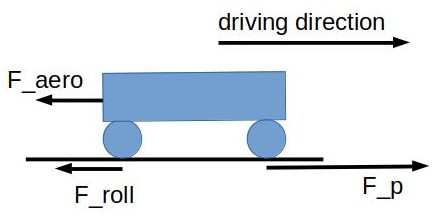
\includegraphics[scale=0.280]{img/physics/flat_road_vehicle_diagram.jpg}
\end{center}
\caption{Schematics of longitudinal forces acting on vehicle.}
\label{flat_road_vehicle_diagram}
\end{figure}

\begin{framed}

\textbf{Remark}

In figure \ref{flat_road_vehicle_diagram}, the vectors have not been drawn to scale. Also, the propulsion force $\mathbf{F}_{p}$ is applied to every motorised wheel however, for simplicity we consider the net or total propulsion force acting on the vehicle. Similarly, the rolling force $\mathbf{F}_{roll}$ represents the total rolling force and not the individual force acting on every wheel. Finally, and in the same vein, the aerodynamic force, $\mathbf{F}_{aero}$,  is the total force acting on the vehicle.

\end{framed}

\begin{framed}

\textbf{Remark}

Forces in the other directions mainly affect the suspension and the steering of the vehicle and we will not consider them here.

\end{framed}

It is easy to understand that $\mathbf{F}_{roll}$ will be zero when the vehicle is not moving. A commonly used model is:


\begin{equation}
\mathbf{F}_{roll}(\alpha) = \left\{
\begin{array}{rl}
	0 & \text{if } v = 0,\\
	\pm c_rmg\cos(\alpha) & \text{if } v \neq 0 
\end{array} \right.
\end{equation}

where 

\begin{itemize}
\item $\alpha$ is the road slope
\item $m$ is the vehicle mass
\item $c_r$ is the rolling resistance coefficient. Typically, is about 0.01 
\item $g$ is the gravitational acceleration constant
\end{itemize}

The rolling resistance force, is approximately independent of the vehicle speed and it exhibits some variation with respect to the road angle. It acts in the opposite direction of the
driving. Thus, it changes sign if the vehicle is moving in the reverse direction. $c_r$ should be as small as possible in order to keep the energy consumption low. 


\section{Questions}


\textbf{Question 1}

Suppose a vehicle is coasting on a flat road, that is, there are no propelling or braking forces acting on the vehicle. This means the only forces that are acting on the vehicle are the rolling resistance and aerodynamic forces. Below you find diagrams describing those forces as a function of vehicle speed

\begin{figure}[!htb]
\begin{center}
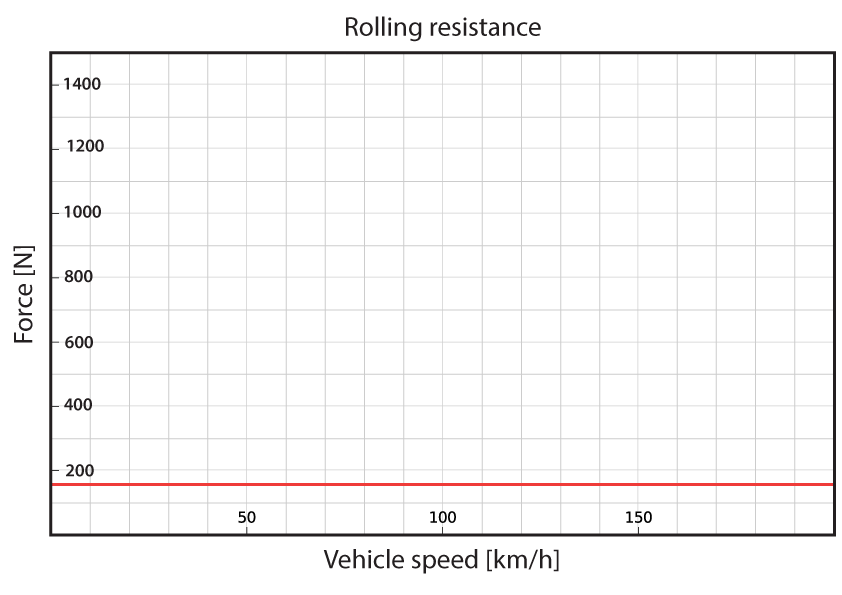
\includegraphics[scale=0.280]{img/physics/Diagram_RollingResistance_01.png}
\end{center}
\caption{Rolling force diagram.}
\label{Diagram_RollingResistance_01}
\end{figure}

\begin{figure}[!htb]
\begin{center}
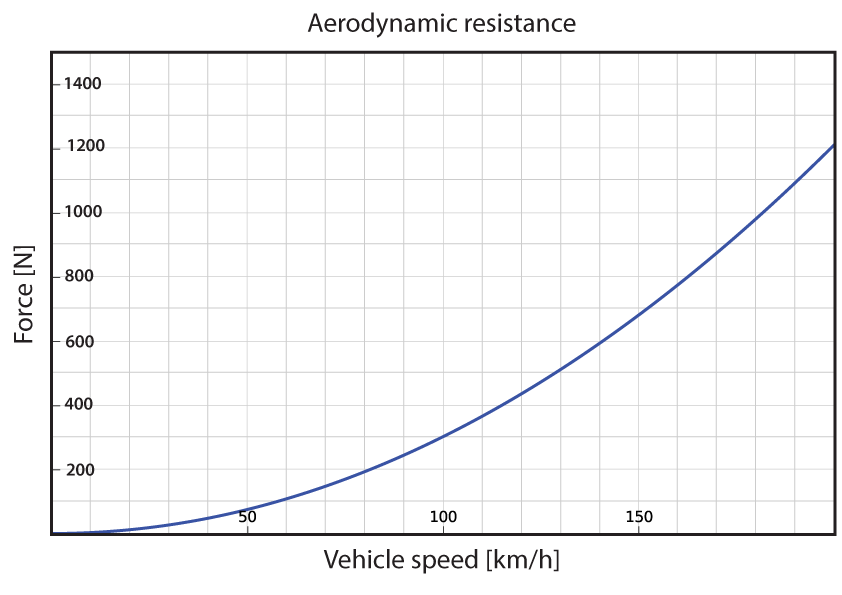
\includegraphics[scale=0.280]{img/physics/Diagram_AerodynamicResistance_01.png}
\end{center}
\caption{Aerodynamics force diagram.}
\label{Diagram_AerodynamicResistance_01}
\end{figure}

What is the sum of the rolling resistance and aerodynamic forces (N) at 100 km/h?


\textbf{Question 2}

Assume the vehicle in question 1 above has the following data:

\begin{tabular}{lll}
\hline
$m$ & 1600\\
$\alpha4$ & 0.0 \\
$A_f$ & 2.1\\
$c_r$ & 0.01\\
$C_D$ & 0.3 \\
$\rho$ & 1.25 \\
$g$ & 9.81 \\
\hline
\end{tabular}

What is the running resistance on a flat road, i e the sum of the rolling resistance and the aerodynamic resistance at 50 km/h? What is the running resistance on a flat road, i e the sum of the rolling resistance and the aerodynamic resistance at 150 km/h?

\textbf{Question 3}

Consider the same vehicle as in Ex.1-2 above. What happens to the resisting forces if the vehicle is made 50\% heavier, but all other parameters remain the same? If the  vehicle front area $A_f$ is increased 10\%, but all other parameters remain the same?








%\chapter{Modeling Automotive Systems}
\label{model_automotive_sys}
In this chapter, we will discuss a number of simplified mathematical models that can be used to model various aspects
of an automobile. Concretely, we will cover the follwoing:

\begin{itemize}
\item Longitudinal vehicle dynamics
\item Drivetrain modeling
\item Suspension modeling
\item Single track model
\end{itemize}

In doing so, we will present and apply a three phase modeling method that comprises of three steps. Namely,

\begin{itemize}
\item Structuring
\item Constitutive relationships
\item State-space model formulation
\end{itemize}
 

\section{Longitudinal Dynamics}
\label{longitudinal_dynamics}
In this section we are interested in developing a model that captures the main longitudinal dynamics of the vehicle. Concretely, we are interested in
how the velocity of the vehicle changes when we press or release the accelerator pedal. We will follow the three phase modeling approach. 

\subsection{Structuring}
Let's assume that the vehicle consists of the powertrain and the chassis. The former produces a propulsion force $\mathbf{F}_p$ that acts on the latter. We can visualize this 
using a block diagram as shown in figure \ref{powertrain_chassis}:

\begin{figure}[!htb]
\begin{center}
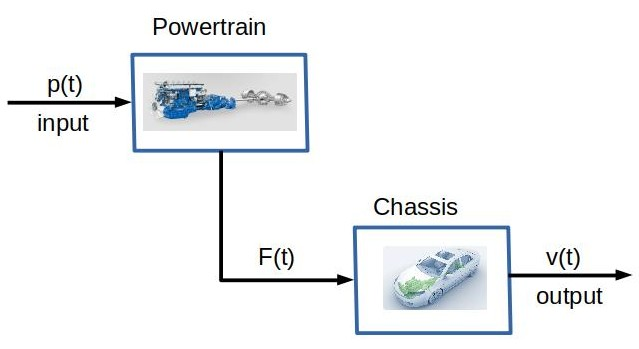
\includegraphics[scale=0.280]{img/model_automotive_sys/powertrain_chassis.jpg}
\end{center}
\caption{Block diagram for powertrain-chassis relationship.}
\label{powertrain_chassis}
\end{figure}

The powertrain can be further broken down into several other subsystems such as:

\begin{itemize}
\item Engine
\item Gearbox
\item Wheels
\end{itemize}

This is shown in the block diagram in figure \ref{engine_gearbox_wheel_block_diagram}


\begin{figure}[!htb]
\begin{center}
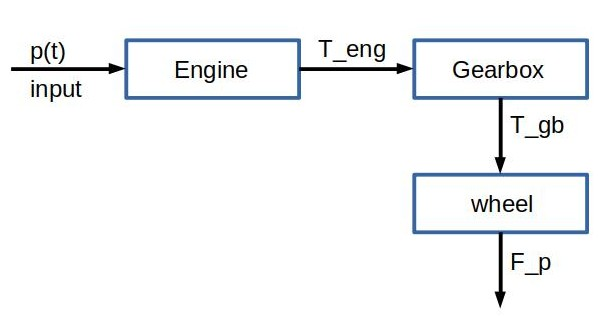
\includegraphics[scale=0.280]{img/model_automotive_sys/engine_gearbox_wheel_block_diagram.jpg}
\end{center}
\caption{Block diagram for engine-gearbox-wheels relationship.}
\label{engine_gearbox_wheel_block_diagram}
\end{figure}



The advantage of such fine grained approach is that we can describe the various components individually. However, the downside is that we increase
the complexity of our model. Hopefully, this increase in complexity will be reflected in an increase of  accuracy of the resulting model.

Let's now start modeling the powertrain. 

\subsection{Powertrain Modeling}

By pressing the pedal, the engine responds by building up a torque $T_{eng}$. We will assume that this build up process can be adequately represented by a first
order dynamics. Thus,

\begin{equation}
\dot{T}_{eng } = - \frac{1}{\tau}T_{eng} + \frac{k}{\tau} p 
\label{engine_model}
\end{equation}

where

\begin{itemize}
\item $p$ is the pedal position
\item $k$ is the steady state gain from the pedal position
\item $\tau$ is the time constant of the engine to build up the torque
\end{itemize}


The gearbox will simply amplify the engine torque, $T_{eng}$,  with a factor equal to the gear ratio $i$ as given by the equation below

\begin{equation}
T_{gb } = iT_{eng} 
\label{gear_model} 
\end{equation}



The wheels convert the torque to force via the wheel radius $r_w$ 

\begin{equation}
\mathbf{F} = \frac{T_{gb}}{r_w}  
\label{wheel_model}
\end{equation}

The wheel model in equation \ref{wheel_model} assumes that there is no slip between the wheels and the ground. 

If we substitute the models \ref{wheel_model} and \ref{gear_model} into \ref{engine_model}, we obtain the following equation for $\mathbf{F}$ which from now on we will call the propulsion force and indicate it instead with $\mathbf{F}_p$


\begin{equation}
\frac{d\mathbf{F}_p}{dt} = - \frac{1}{\tau}\mathbf{F}_p + \frac{ki}{\tau r_w} p   
\label{engine_model_II}
\end{equation}

\subsection{Chassis Modeling}
The propulsion force, $\mathbf{F}_p$, produced by the powertrain can be given as an input to the chassis model as shown schematically in figure

 
\begin{figure}[!htb]
\begin{center}
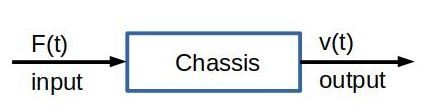
\includegraphics[scale=0.280]{img/model_automotive_sys/chassis_block_diagram.jpg}
\end{center}
\caption{Block diagram for chassis component.}
\label{chassis_block_diagram}
\end{figure}

We can derive the governing equation describing the dynamics of the chassis by using Newton's law:

\begin{equation}
m\mathbf{a} =  \mathbf{F}_T 
\label{chassis_force_balance}
\end{equation}

where $m$ is the vehicle mass and $\mathbf{F}_T$ is the total or net force acting on the chassis. The net force is assumed to have the following components 

\begin{itemize}
\item $\mathbf{F}_p$ propulsion force
\item $\mathbf{F}_{aero}$ aerodynamic force coming from the movement of the vehicle
\item $\mathbf{F}_{grav}$ the graviational force
\item $\mathbf{F}_{roll}$ the rolling resistance force
\end{itemize}

Thus,

\begin{equation}
\mathbf{F}_T = \sum_{i} \mathbf{F}_i =  \mathbf{F}_p -  \mathbf{F}_{aero} - \mathbf{F}_{grav} -  \mathbf{F}_{roll}
\label{chassis_model_total_force}
\end{equation}

The propulsion force is assumed to act in the direction of motion and must be large enough to overcome the three other forces in order for
the vehicle to able to move. The following body diagram illustrates this.


\begin{figure}[!htb]
\begin{center}
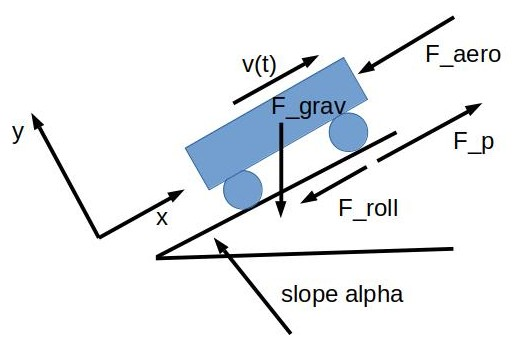
\includegraphics[scale=0.280]{img/model_automotive_sys/free_diagram_chassis.jpg}
\end{center}
\caption{Chassis free body diagram.}
\label{free_diagram_chassis}
\end{figure}

Note that in the figure above the propulsion and rolling forces are only shown to act in one wheel which is not true.

Since we assume that the road has slope $\alpha$,  it useful to decompose the forces in the $x$ and $y$ direction:


\begin{eqnarray}
x: m\alpha_x = F_{p, x} - F_{aero,x} - F_{grav, x} - F_{roll, x}  \\
y: m\alpha_y = F_{p, y} - F_{aero,y} - F_{grav, y} - F_{roll, y}  \\
\label{chassis_model_force_decomp}
\end{eqnarray}


\subsection{Balance Laws \& Constitutive Equations}

Let's now turn attention to the constitutive equations. Ideally, we would not like to have any accelerations in the $y$ direction thus $\alpha_y =0$. Furthermore, there in no drag force component
in the in the $y$ direction; $F_{aero,y} = 0$ whilst the drag term in the $x$ direction is modelled via:

\begin{equation}
F_{aero,x} = \frac{1}{2}\rho C_D A_f v^2 
\label{chassis_model_drag_term}
\end{equation}

where

\begin{itemize}
\item $\rho$ is the air density
\item $C_D$ is the drag coefficient
\item $\mathbf{F}_{grav}$ the graviational force
\item $\mathbf{F}_{roll}$ the rolling resistance force
\end{itemize}

From figure \ref{gravity_decomp_diagram}


\begin{figure}[!htb]
\begin{center}
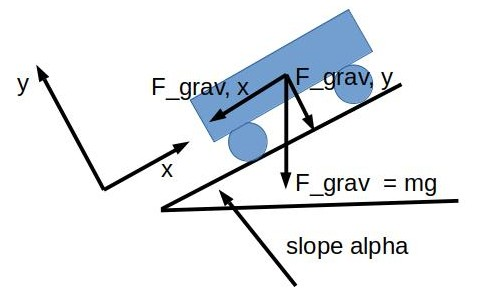
\includegraphics[scale=0.280]{img/model_automotive_sys/gravity_decomp_diagram.jpg}
\end{center}
\caption{$\mathbf{F}_{grav}$ force decomposition.}
\label{gravity_decomp_diagram}
\end{figure}


we can decompose the $\mathbf{F}_{grav}$ into 

\begin{eqnarray}
x: F_{grav, x} = mg\sin(\alpha)  \\
y: F_{grav, y} = mg\cos(\alpha) 
\label{gravity_decomp}
\end{eqnarray}

Finally, the rolling force in the x-direction $F_{roll, x}$ is modelled as a fraction of the vehicle load:

\begin{equation}
F_{roll,x} = (N_1 + N_2)f
\label{chassis_model_roll_force}
\end{equation}


\subsection{Summary Of Balance Laws \& Constitutive Equations}
Let's now summarize the equations and constitutive relations used for our model. Note that the acceleration $\boldsymbol{\alpha}$  is given by

\begin{eqnarray}
\boldsymbol{\alpha} = \frac{d \mathbf{v}}{dt}
\label{acceleration_vel_relationship}
\end{eqnarray}

\begin{itemize}
\item Chassis dynamics 
\end{itemize}

\begin{eqnarray}
x: m\alpha_x = F_{p, x} - F_{aero,x} - F_{grav, x} - F_{roll,x}  \\
y: 0 = N_1 + N_2 - F_{grav, y} 
\label{chassis_model_summary}
\end{eqnarray}

where

\begin{itemize}
\item $F_{aero,x} = \frac{1}{2}\rho C_D A_f v^2 $ 
\item $F_{grav, x} = mg \sin(\alpha)$ 
\item $F_{grav, y} = mg \cos(\alpha)$ 
\item $F_{roll,x} = (N_1 + N_2)f$ the graviational force
\item $N_1,  N_2$ are the vehicle load on the back and front wheels respectively 
\end{itemize}

The propulsion force $\mathbf{F}_p$ is given by the solution of

\begin{equation}
\frac{d\mathbf{F}_p}{dt} = - \frac{1}{\tau}\mathbf{F}_p + \frac{ki}{\tau r_w} p   
\label{engine_model_III}
\end{equation}


\subsection{State-Space Form}
We will now cast the model above into the state-space form. The first step is to select the state variables. We do so by observing what changes. We have two items here

\begin{itemize}
\item The propulsion force $\mathbf{F}_p$  
\item The velocity $\mathbf{v}$
\end{itemize}


\section{Questions}

\textbf{Question 1}

Consider the the longitudinal motion vehicle model

\begin{eqnarray}
\frac{dx_1}{dt} = \frac{1}{\tau}x_1 + \frac{ki}{\tau r_w} u \nonumber \\
\frac{dx_2}{dt} = \frac{1}{m} \left ( x_1 - mgf\cos(\alpha) - \frac{1}{2}\rho C_DA_f x_{2}^2 - mg\sin(\alpha) \right )  \nonumber \\
y = x_2 \nonumber
\end{eqnarray}

where  $x-1$ is the force at the wheels, $x_2$ is the vehicle velocity, $u$ is the input signal, the accelerator pedal position, and $\alpha$ is the disturbance, the road slope.

Is the longitudinal vehicle dynamics model linear?

Is the longitudinal vehicle dynamics model time invariant?

Determine the required engine torque (Nm) for a vehicle acceleration of 0.3 $m/s^2$ on a flat road at 60 $km/h$!


Longitudinal slip is the relative motion between a tire and the road surface it is moving on: 

\begin{equation}
\text{slip} = \frac{r_w \omega - v}{v}
\end{equation}

which means that the wheels are spinning if slip is positive and that the wheels are skidding if slip is negative. The longitudinal vehicle dynamics model is developed under the assumption that the relative motion between the tire and the road surface is zero, i.e. is not included in the model.

If we would like to include slip into our model, how many additional states are needed in order to include longitudinal slip into the model?


One additional state is needed as we need to include the wheel speed as an additional state variable in order to capture slip as we already have velocity as one state. 

When performing numerical simulations with the longitudinal vehicle dynamics model including the slip model, you might run into numerical problems. Why?

\begin{itemize}
\item A) Division by zero, due to zero velocity 
\item B) Division by zero, due to zero wheel speed 
\item C) Division by zero, due to zero engine torque 
\end{itemize}

The slip model includes a normalization with respect to the vehicle velocity. This gives numerical problems when the velocity is zero, i.e. division by zero. Thus, option A is the correct answer.


\section{Drivetrain Modeling}

\section{Suspension System Modeling}

In this section we will derive a mathematical model for the vehicle suspension system. Concretely, we will assume a passive suspension system.


\begin{framed}

\textbf{Active and Passive Suspension System}

Active suspension is a type of automotive suspension that controls the vertical movement of the wheels relative to the chassis or vehicle body with an onboard system, rather than in passive suspension where the movement is being determined entirely by the road surface. Active suspensions can be generally divided into two classes: 

\begin{itemize}
\item pure active suspensions, 
\item adaptive/semi-active suspensions. 
\end{itemize}
While adaptive suspensions only vary shock absorber firmness to match changing road or dynamic conditions, active suspensions use some type of actuator to raise and lower the chassis independently at each wheel. For more information see the Wikipedia entry: https://en.wikipedia.org/wiki/Active\_suspension

\end{framed}


The suspension system connects the vehicle body with the wheels. furthermore, it gives the whell a vertical movement possibility. A common approach to model the vehicle suspension
system is to consider only one of the four wheels. The schematic of a simplified suspension system is shown in figure

For a passive suspension system, the input is road surface $z_r$. The outputs will be the positions of the wheels $z_w$ and that of the chassis $z_c$. The block diagram is shown in figure
\ref{suspension_sys_block_diagram} 

\begin{figure}[!htb]
\begin{center}
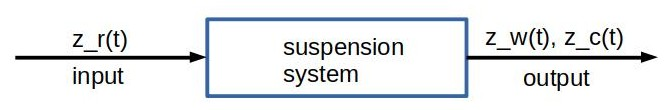
\includegraphics[scale=0.280]{img/model_automotive_sys/suspension_sys_block_diagram.jpg}
\end{center}
\caption{Block diagram for suspension system.}
\label{suspension_sys_block_diagram}
\end{figure}

The free body diagram for the wheel mass is shown in figure \ref{suspension_sys_wheel_mass_free_diagram}


\begin{figure}[!htb]
\begin{center}
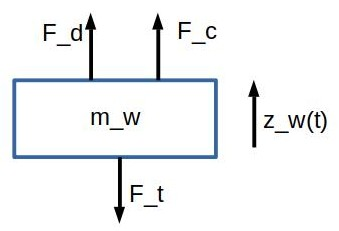
\includegraphics[scale=0.280]{img/model_automotive_sys/suspension_sys_wheel_mass_free_diagram.jpg}
\end{center}
\caption{Wheel mass free body diagram.}
\label{suspension_sys_wheel_mass_free_diagram}
\end{figure}

where $\mathbf{F}_t$ is the tire force, $\mathbf{F}_d$ is the suspension force and $\mathbf{F}_c$ is the chassis force. Similarly, the free body diagram for the chassis mass is shown in figure \ref{suspension_sys_wheel_mass_free_diagram}

\begin{figure}[!htb]
\begin{center}
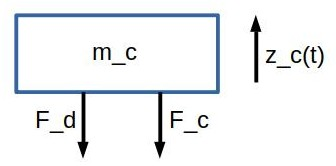
\includegraphics[scale=0.280]{img/model_automotive_sys/suspension_sys_chassis_mass_free_diagram.jpg}
\end{center}
\caption{Chassis mass free body diagram.}
\label{suspension_sys_chassis_mass_free_diagram}
\end{figure}


\section{The Bicycle Model}
\label{bicycle_model}

We would like to be able to control the vehicle; for example when following a predefined path or when making an avoidance manouver. These types of motions
require control of the lateral dynamics that the longitudinal model developed in section \ref{longitudinal_dynamics} does not account for. We would like therefore
to generalize somehow our model.

Thus, in  this  section,  we  study the kinematic bicycle model, which is often used for trajectory planning,  
and  compare  its  results  to  a  none  degrees  of  freedom model. Modeling errors and limitations of the kinematic bicycle model are highlighted. 

The three degrees of freedoom (DOFs) kinematic bicycle model, see figure \ref{bicycle_model_1},  is one
of the simplest models frequently used at the motion planning phase, with the belief that it is able to capture enough of the
nonholonomic constraints of the actual vehicle dynamics. By constrast, even relatively simple vehicle models used for low level  control  can  imply  more  
than  ten DOFs \cite{Polack2017}. 


\begin{figure}[!htb]
\begin{center}
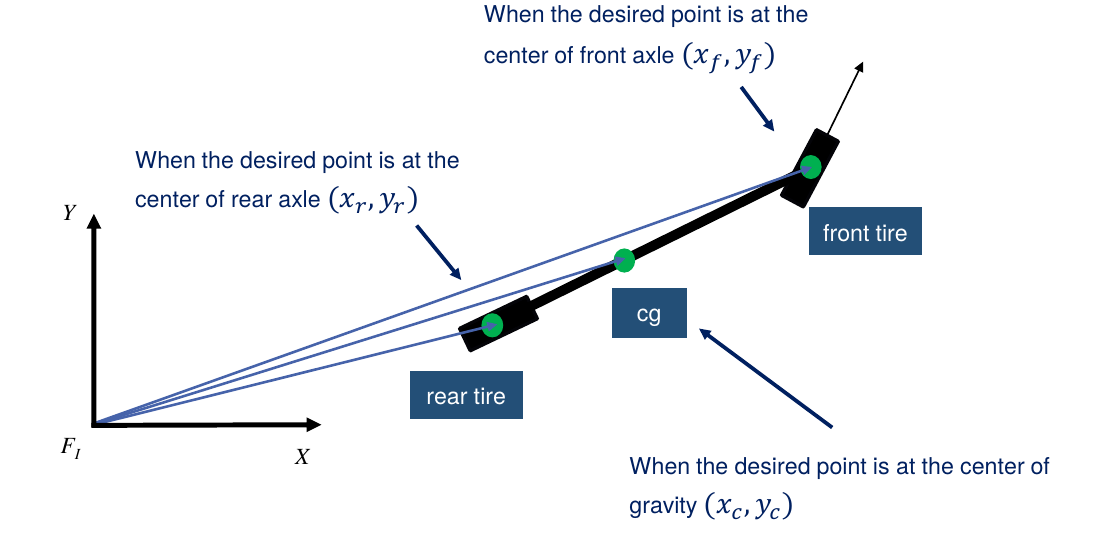
\includegraphics[scale=0.290]{img/model_automotive_sys/bicycle_model_1.jpeg}
\end{center}
\caption{Schematic of the bicycle model.}
\label{bicycle_model_1}
\end{figure}


In the kinematic bicycle model, the two front wheels (respectively the two rear wheels) of the vehicle are lumped into a unique
wheel  located  at  the  center  of  the  front  axle  (respectively  of  the rear axle) such as illustrated on Figure 1. 
The control inputs correspond to the acceleration $\boldsymbol{\alpha}$ and the front wheel steering angle $\delta$
of  the  vehicle,  when  assuming  that  only  the  front wheel can be steered. The kinematic bicycle model can then



%\chapter{Linear Systems}
\label{linear_systems}
Modeling of automotive systems (or any other system whatsoever) typically results in a mathematical description of it. This mathematical description is usually given in the
form of differential equations that involve the input(s) and the output(s) of the system as well as other parameters that are of interests and affect its behavior. In this chapter,
we introduce the notion of a linear system (LS) and other useful terms that will be used in subsequent chapters. We will see that a LS can be represented in different forms susch as:


\begin{itemize}

\item Differential equations
\item Transfer functions
\item State-Space models

\end{itemize} 

\section{Linear ODEs}

Let's consider the ODE:

\begin{equation}
\frac{d^{n}y}{dt^{n}} + \alpha_{1}\frac{d^{n-1}y}{dt^{n-1}} + \dots + \alpha_{n}y = \beta_{1}\frac{d^{n-1}u}{dt^{n-1}} + \dots + \beta_{n}u  
\label{linear_sys_1}
\end{equation}

where $u$ represents the input to the system and $y$ represents the output. $\alpha_i$ and $\beta_i$ are coefficients which may or may not be time dependent. In the case that the coefficients do not depend on
the time variable $t$ we have a linear time invariant (LTI) system. Otherwise the system will be time variant.


\begin{framed}

\textbf{Superposition Principle}

Let the linear equation:

\begin{equation}
L{y} = F(x)
\end{equation}

where $L$ is a linear operator. If $y_1$ and $y_2$ are solution of the linear equation, then their sum will also be a solution.

\end{framed}

Every solution to such a system can be written as the sum (because the system is linear superposition of solutions...) of a solution $y_h$to the homogeneous equation and a particular solution $y_p$:


\begin{equation}
y = y_h + y_p
\label{linear_sys_general_sol}
\end{equation}

The solution to the homogeneous solution will have the form:

\begin{equation}
y_h = \sum_{k=1}^{n} C_k e^{s_k t}  
\label{linear_sys_general_ho}
\end{equation}

where $s_k$ are the roots of the so called characteristic equation or polynomial (see section \ref{characteristic_equation}) and  $C_k$ can be determined from the initial conditions. 


Now that we have established the general form of the homogeneous
solution, let's turn our attention to the particular solution.  In order to find the particular solution $y_p$, we need the input signal $u$. Let's assume a damped sinusoidal input signal of the following form

\begin{equation}
u(t) = e^{st}  
\label{linear_sys_input}
\end{equation}

where $s$ is a complex variable.  The particular solution is assumed to have the follwoing general form:


\begin{equation}
y_p= G(s)e^{st}  
\label{linear_sys_general_pa}
\end{equation}

The function $G(s)$ is called the transfer function TF. Thus, the general solution of the equation \ref{linear_sys_1} is


\begin{equation}
y (t) = \sum_{k=1}^{n} C_k e^{s_k t} + G(s)e^{st}  
\label{linear_sys_general_sol_II}
\end{equation}

The first part gives the dependency due to the initial conditions. The second part is due to the input signal.


\subsection{Characteristic Equation}
\label{characteristic_equation}

In equation \ref{linear_sys_general_sol_II} the $s_k$s are the roots of the characteristic equation or polynomial $\alpha(s)$. This polynomial is formed from the coefficients of the system
\ref{linear_sys_1}. Hence, for the system

\begin{equation}
\frac{d^{n}y}{dt^{n}} + \alpha_{1}\frac{d^{n-1}y}{dt^{n-1}} + \dots + \alpha_{n}y = \beta_{1}\frac{d^{n-1}u}{dt^{n-1}} + \dots + \beta_{n}u  
\nonumber
\end{equation} 

we will have

\begin{equation}
\alpha(s) = s^n +\alpha_{1}s^{n-1} + \dots + \alpha_n   
\label{linear_sys_charact_pol}
\end{equation}
Thus, the $s_k$ will be the roots of the equation


\begin{equation}
\alpha(s) = 0 
\label{linear_sys_charact_pol_eq}
\end{equation}

Concretely, the solutions $s_k$ are called the \textbf{poles}  of the system and play a crucial role in the stability of the solution:

\begin{itemize}
\item If all the roots of $\alpha(s)=0$ have $Re(s_k) < 0 $ then the system is asymptotically stable
\item If any of the roots of $\alpha(s)=0$ has $Re(s_k) > 0 $ then the system is  unstable
\end{itemize}

\begin{framed}
\label{linear_sys_exe_1}

\textbf{Example}

Consider the system

\begin{equation}
\dot{x} = x +u \nonumber
\end{equation}

Form the characteristic equation. Is the solution stable or not?

\textbf{Answer}

The characteristic equation of the system above is

\begin{equation}
\alpha(s) = s -1 =0 \nonumber
\end{equation}

The only root to this equation is $s=1$ and since $Re(s) > 0$ the system is not asymptotically stable.

\end{framed}



\subsection{Laplace Transformation}


\section{State-Space models}

A state-space formulation of a linear system has the following form



\begin{eqnarray}
\dot{x} = Ax + Bu \\
y = Cx + Du
\label{linear_space_form}
\end{eqnarray}

where

\begin{itemize}
\item $x \in R^{n}$ is the state vector
\item $y \in R^{n}$ is the output vector
\item $u \in R^{p}$ is the input vector 
\item $A \in R^{n \times n}$ is the matrix describing the dynamics 
\item $B \in R^{n \times p}$ is the matrix describing the input 
\item $C \in R^{q \times n}$ is the output or sensor matrix 
\item $D \in R^{q \times p}$ is the direct matrix 
\end{itemize}

Just like in equation \ref{linear_sys_1}, if the coefficient matrices do not depend on time, we have an LTI system.



\section{Questions}


\textbf{Question 1}

Consider the following model:

\begin{equation}
\dot{x} = x +u \nonumber
\end{equation}

We saw in example \ref{linear_sys_exe_1} that the solution to this system is asymptotically stable. Cast the system in the

\begin{equation}
\frac{dx}{dt} = Ax + Bu \nonumber
\end{equation}

form and argue again about its stability.


\textbf{Answer}

We can write the given system in the form above if we assume that

\begin{equation}
A = [1] ~~ \text{and} ~~ B = [1]  \nonumber
\end{equation}

The stability depends on the eignevalues of $A$ and  here we have only one eigenvalue which is $\lambda = 1$. Thus, since $Re(\lambda) > 0 $ the system is not asymptotically stable as we concleded in example 
\ref{linear_sys_exe_1}


\textbf{Question 2}

Consider the following model:

\begin{equation}
\frac{d^2x}{dt^2} + 2\frac{dx}{dt} + x  = u \nonumber
\end{equation}

compute the poles of the equation and argue about the stability.


\textbf{Answer}

The poles of the equation are the solutions of the characteristic equation:

\begin{equation}
\alpha(s) = s^2 + 2s +1 =0  \nonumber
\end{equation}

The discriminant of the quadratic equation is

\begin{equation}
\Delta = b^2 - 4ac =0  \nonumber
\end{equation}

Hence, the characteristic polynomial has only one real solution given by

\begin{equation}
s = \frac{-b}{2a} = -1  \nonumber
\end{equation}

Thus, since $Re(s) < 0 $ the system is asymptotically stable.



\textbf{Question 3}

Determine the poles of the following equations:


\begin{eqnarray}
\text{A)} ~~ \frac{d^2x}{dt^2} + 2\frac{dx}{dt} + x = u \nonumber \\
\text{B)} ~~ \frac{d^2x}{dt^2} + 2\frac{dx}{dt} + 2x = u \nonumber \\
\text{C)} ~~ \frac{d^2x}{dt^2} + 3\frac{dx}{dt} + 2 x  = u \nonumber \\
\end{eqnarray}


For the the model A we have:

\begin{equation}
\alpha(s) = s^2 + 2s +1 =0  \nonumber
\end{equation}

Thus, only one pole $s=-1$. For model B,

\begin{equation}
\alpha(s) = s^2 + 2s +2 =0  \nonumber
\end{equation}

The discriminant $\Delta = -4 <0$.  Thus, the system has two complex solution

\begin{eqnarray}
s_1 = -1 +i  \nonumber \\
s_2 = -1 -i  \nonumber \\
\end{eqnarray}

For model C, 

\begin{equation}
\alpha(s) = s^2 + 3s +2 =0  \nonumber
\end{equation}

and the solutions are

\begin{eqnarray}
s_1 = -1   \nonumber \\
s_2 = -2  \nonumber \\
\end{eqnarray}









%\chapter{Examples I}
\label{examples_I}
In this chapter we will present some examples in order to reinforce and clarify various topics introduced in the previous chapters

\section{PI Cruise Controller}
In this example we will analyse the model of the closed loop cruise controller. This is shown in the image below


\begin{figure}[!htb]
\begin{center}
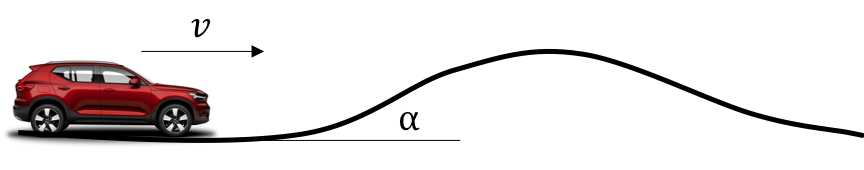
\includegraphics[scale=0.380]{img/model_based_eng/P1_1_2_1_ex_2.png}
\end{center}
\caption{Schematics of PI close loop cruise controller.}
\label{P1_1_2_1_ex_2}
\end{figure}

\begin{figure}[!htb]
\begin{center}
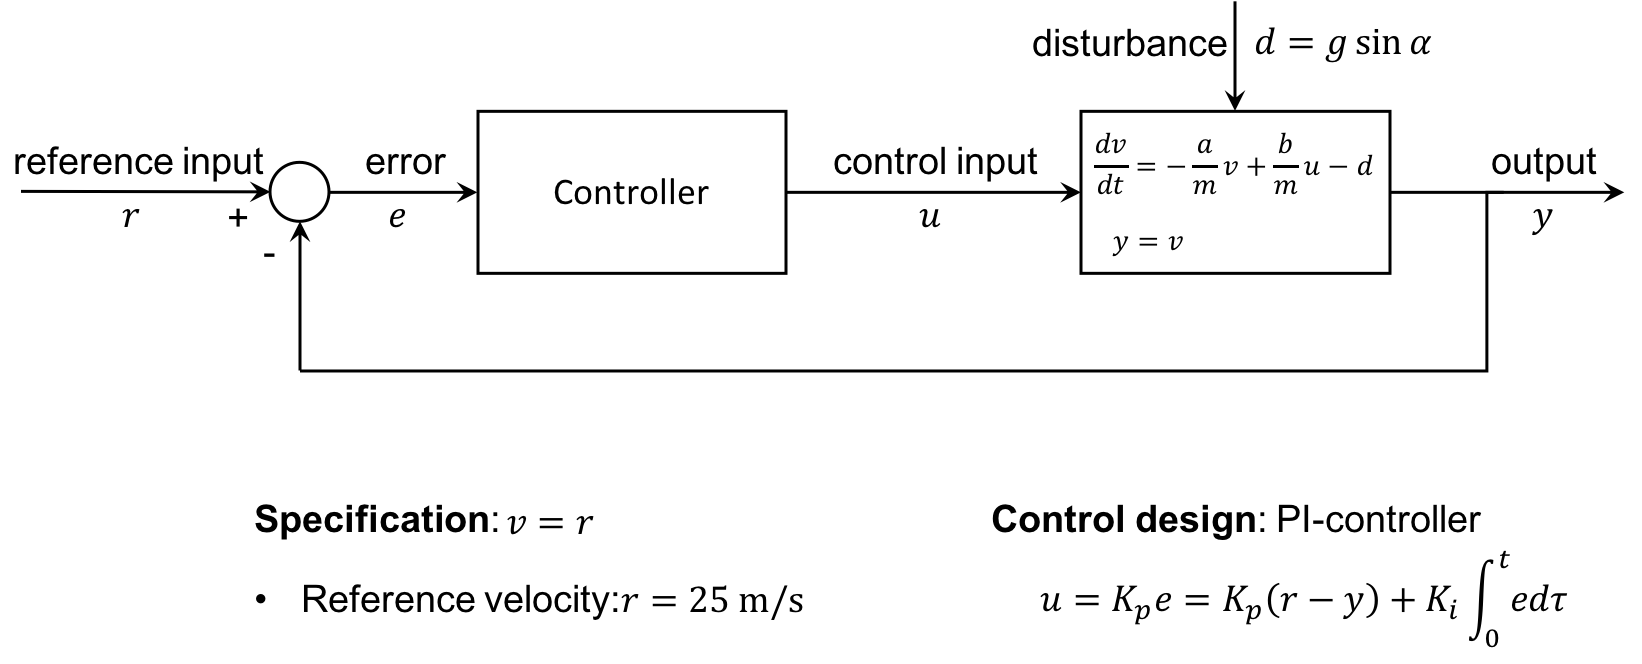
\includegraphics[scale=0.280]{img/model_based_eng/P2_1_2_1_ex_2_cruise.png}
\end{center}
\caption{Schematics of PI close loop cruise controller.}
\label{P2_1_2_1_ex_2_cruise}
\end{figure}


\subsection{Questions}

\textbf{Question 1:}

Which features are representative for a closed loop controller?

\begin{itemize}
\item A) Acts on deviation
\item B) No risk for instability
\item C) Risk for instability
\item D) Insensitive to measurement noise 
\end{itemize}

\textbf{Answer:}
A closed loop controller acts on the deviation from the reference signal in a measure-decide-act cycle. So 
option A is correct. Closed loop controllers are subject to instability problems; the closed loop dynamics can be shaped in such a way that the system might become unstable. So option C is also correct.


\textbf{Question 2:}

Which features are representative for an open loop controller?

\begin{itemize}
\item A) Acts on deviation
\item B) No risk for instability
\item C) Risk for instability
\item D) Insensitive to measurement noise 
\end{itemize}

\textbf{Answer:}
In an open loop controller all control actions are preprogrammed (otherwise we have no control). Thus, option A is correct. Option B is also correct provided that the system is also stable. In this case the open loop controller will also be stable. For an open loop controller no measurements are required, so no sensitivity towards measurements (VERIFY THIS). Thus, option D is also correct. 


\textbf{Question 3:}

Would you say that a driver is closed loop or open loop controller? 

\textbf{Answer:}
Since a driver typically aquires feedback via his/her senses and acts accordingly in order to adapt to the measured feedback, we can say that a driver is a closed loop controller.





\section{Output Feedback}
\label{output_feedback}

Chapter \ref{state_feedback} introduced the concept of reachability. It was shown that it is possible to find 
a state feedback law that gives the desired closed loop eigenvalues provided that the system
is reachable.  Furthermore, we saw how to design controllers using
the system state, $x(t)$, as feedback to out controller. 

However, desigining state feedback controllers preassumes that all the states are measured. For many situations, it
is highly unrealistic to assume that all the states are measured. 

In this section we proceed somehow in a similar vein we can use the output $y(t)$ to modify the dynamics of the system through the use of observers. Furthermore, we will introduce the concept of observability
and show that if a system is observable, it is possible to recover the state
from measurements of the inputs and outputs to the system. We then show how to
design a controller with feedback from the observer state. 




\section{Observability}
\label{observability}

For many situations, it is highly unrealistic to assume that all the states are measured. In this section we
investigate how the state can be estimated by using a mathematical model and a
few measurements. It will be shown that computation of the states can be carried
out by a dynamical system called an \textbf{observer}, see also figure \ref{observer_block_diagram}.


\begin{framed}
\theoremstyle{definition}
\begin{definition}{\textbf{Observability}}
A linear system is \textbf{observable}  if for any $T>0$ it is possible to determine the state of the system $x(T)$ through measurements of $y(t)$ and $u(t)$ on the interval $[0,T]$  $x(T) = x_f$.
\end{definition}
\end{framed}


\begin{framed}
\theoremstyle{remark}
\begin{remark}{\textbf{Nonlinear Systems}}

The definition above holds for nonlinear systems as well, and the results discussed here have extensions to the nonlinear case.
\end{remark}
\end{framed}


Consider again the system

\begin{equation}
\frac{dx}{dt} = Ax + Bu ~~ y = Cx + Du
\end{equation}


where $x\in R^n$ is the state, $u\in R^{p}$ is the input and $y\in R^q$ the measured output.

We wish to estimate the state of the system from its inputs and outputs, as illustrated
in Figure \ref{observer_block_diagram}. In some situations we will assume that there is only one measured
signal, i.e., that the signal $y$ is a scalar and that $C$ is a (row) vector. This signal may
be corrupted by noise $n$, although we shall start by considering the noise-free case.
We write $\hat{x}$ for the state estimate given by the observer.

\begin{figure}[!htb]
\begin{center}
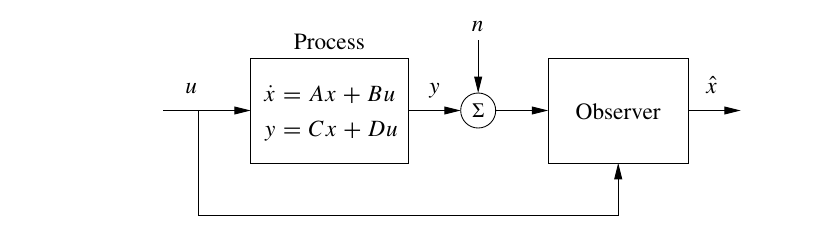
\includegraphics[scale=0.380]{img/output_feedback/observer_block_diagram.jpeg}
\end{center}
\caption{Block diagram for an observer. The observer uses the process measurement $y$
(possibly corrupted by noise $n$) and the input $u$ to estimate the current state of the process,
denoted $\hat{x}$.}
\label{observer_block_diagram}
\end{figure}


The problem of observability is one that has many important applications, even
outside feedback systems. If a system is observable, then there are no hidden dynamics inside it; we can understand everything that is going on through observation (over time) of the inputs and outputs. As we shall see, the problem of observability is of significant practical interest because it will determine if a set of sensors is
sufficient for controlling a system. Sensors combined with a mathematical model
can also be viewed as a virtual sensor that gives information about variables that
are not measured directly. The process of reconciling signals from many sensors
with mathematical models is also called sensor fusion.



\section{Testing for Observability}
\label{test_observability}

When discussing reachability in the last chapter, we neglected the output and focused on the state. Similarly, it is convenient here to initially neglect the input and
focus on the autonomous system



\begin{framed}
\theoremstyle{remark}
\begin{remark}{\textbf{Autonomous System}}

\end{remark}
\end{framed}

\begin{equation}
\frac{dx}{dt} = Ax ~~ y = Cx
\end{equation}

The objective is to understand when it is possible to determine the state from observations of the output. From

\begin{equation}
y = Cx
\end{equation}

we see that the output itself gives us the projection of the state $x$ on vectors that are rows of the matrix $C$. The 
observability problem can  immediately be solved if the matrix $C$ is invertible. If the matrix is not invertible we can take the derivatives and obtain

 
\begin{equation}
\frac{dy}{dt} = C\frac{dx}{dt} = CAx
\end{equation}

From the derivative of the output we thus get the projection of the state on vectors that are rows of the matrix $CA$. Proceeding in this way, we get

\begin{equation}
\begin{bmatrix}
 y \\
 y^{(1)} \\
 \vdots \\
 y^{(n-1)} 
\end{bmatrix} = 
\begin{bmatrix}
 C \\
 CA \\
 \vdots \\
 CA^{n-1} 
\end{bmatrix}x
\end{equation}

We thus find that the state can  be  determined if the observability matrix
 
\begin{equation}
W_o= 
\begin{bmatrix}
 C \\
 CA \\
 \vdots \\
 CA^{n-1} 
\end{bmatrix}
\end{equation}

has $n$ independent rows.  It turns out  that  we  need  not consider any derivatives higher
than $n-1$ (this is an application of the Cayley-Hamilton theorem)
 
\begin{framed}
\theoremstyle{remark}
\begin{remark}{\textbf{System with inputs}}

The calculation can easily be extended to systems with inputs. The state is then
given by a linear combination of inputs and outputs and their higher derivatives.
The observability criterion is unchanged. 
\end{remark}
\end{framed}


\begin{framed}
\theoremstyle{theorem}
\begin{theorem}{\textbf{Observability rank condition}}

A linear system of the form  
\begin{equation}
\frac{dx}{dt} = Ax + Bu, ~~ y = Cx + Du \nonumber
\end{equation}

is observable if and only if the observability matrix $W_o$ is full rank.
\end{theorem}
\end{framed}

\section{Observable Canonical Form}
\label{observability_canonical_form}

As in the case of reachability, certain canonical forms will be useful in studying ob-
servability. A linear single-input, single-output state space system is in observable
canonical form if its dynamics are given by


\begin{framed}
\theoremstyle{remark}
\begin{remark}{\textbf{Observable Canonical Form for Nonlinear Systems}}

The definition can be extended to systems with many inputs; the only difference is
that the vector multiplying u is replaced by a matrix.
\end{remark}
\end{framed}


The characteristic polynomial for a system in observable canonical form is

\begin{equation}
\lambda(s) = s^n +\alpha_1s^{n-1} + \ldots + \alpha_{n-1}s + \alpha_n
\end{equation}

In order to check the observability property of a systme more formally, we can compute the observability matrix for
a system in observable canonical form. This is given by

\begin{equation}
W_o= 
\begin{bmatrix}
 1 & 0 & 0 & \ldots &  0\\
 -\alpha_1 & 1 & 0 & \ldots &  0 \\
 -\alpha_{1}^{2} - \alpha_1 \alpha_2 & - \alpha_1 & 1 &  \ldots &  0 \\
 \vdots & \vdots & \vdots & \ddots & \vdots \\
* & * & * & \ldots & 1
\end{bmatrix} 
\end{equation}


where * represents  an entry  whose exact  value  is  not important.
What is important here is the rows of this matrix are linearly independent (since it is lower triangular), and hence Wo is full rank. Hence, it is invertible. 

As in the case of reachability (see section \ref{reachable_canonical_form}), it  turns  out  that  if a  system  is  observable then there
always exists a transformation $T$ that converts the system into observable canonical
form. This is useful for proofs since it lets us assume that a system is in observable
canonical form without any loss of generality. The observable canonical form may
be poorly conditioned numerically.
 

\section{State Estimation}
State feedback control design, as explained in t chapter \ref{state_feedback} requires that we have access to the complete state vector. 
However, measuring the complete state vector is not always feasible (for example a sensor may not be available at all) and it may also be expensive.
In this section we will introduce the idea of state estimation as a way to get access to the state variables. 


\begin{framed}
\theoremstyle{remark}
\begin{remark}{\textbf{Soft Sensors}}


The concept of using software instead of sensors to access the quantity we are 
interested in, is referred to as soft sensors in the automotive industry.
\end{remark}
\end{framed}

Recall that the idea of state feedback control was to modify the eigenvalues of the system under consideration by using the input

\begin{equation}
u = -Kx + K_r r  
\end{equation}

However, it can be seen that this requires the state vector $x$. The idea of state estimation is to design something called an observer that tries to provide an 
estimate say $\hat{x}$ of the state vector $x$. The observer is fed with the same input as the real plant. The goal of the observer is to provide somehow a replica of the true state vector.
Thus, we would like to have the error $\tilde{x}$ between the two quantities to be zero. Namely,


\begin{equation}
\tilde{x} = x - \hat{x} = 0 
\end{equation}
 
In this section, we want to construct a dynamical system of the form

\begin{equation}
\frac{d \hat{x}}{dt} = F\hat{x} + Gu + Hy  
\end{equation}

where $u$ and $y$ are the input and output of the original system and $\hat{x} \in R^n$ is an estimate of $x$ with the property

\begin{equation}
\hat{x}(t) \rightarrow x(t), ~~ \text{as} ~~ t \rightarrow \infty  
\end{equation}

Let's consider again the system

\begin{equation}
\frac{dx}{dt} = Ax + Bu ~~ y = Cx + Du
\label{sys}
\end{equation}

assume further that $D$ is zero. Assuming that the input $u$ is known, then an estimate of the state $x$ is given by

\begin{equation}
\frac{d\hat{x}}{dt} = A\hat{x} + Bu
\label{observer_one} 
\end{equation}  

We would like to know the properties of this estimate; how far is from the exact state? The estimation error is \cite{Astrom} 

\begin{equation}
\tilde{x} = x - \hat{x} 
\end{equation} 

substituting into equation \ref{observer_one} we find that


\begin{equation}
\frac{d\tilde{x}}{dt} = A\tilde{x}  
\end{equation}  

We already know that the behavior of this system depends on the eigenvalues of $A$. Concretely, if matrix $A$ has all its eigenvalues in the left half-plane, the error $\tilde{x}$ will go to zero,
and hence equation \ref{observer_one} is a dynamical system whose output converges to the state
of the system \ref{sys}.


The observer given by equation \ref{observer_one} uses only the process input $u$; the measured
signal does not appear in the equation. We must also require that the system be stable,
and essentially our estimator converges because the state of both the observer and
the estimator are going zero. This is not very useful in a control design context since
we want to have our estimate converge quickly to a nonzero state so that we can
make use of it in our controller. We will therefore attempt to modify the observer
so that the output is used and its convergence properties can be designed to be fast
relative to the system’s dynamics. This version will also work for unstable systems.

Let's now consider the following observer

\begin{equation}
\frac{d \hat{x}}{dt} = A\hat{x} + Bu + L(y- C \hat{x})
\label{observer_two}   
\end{equation}

The term $L(y- C \hat{x})$ provides feedback and hence the observer in \ref{observer_two} can be seen as a generalization of the observer in \ref{observer_one}. The supplied feedback is proportional to the difference between the observed output and the output predicted by the observer. Substituting the expression for the error $\tilde{x}$ we arraive at

 \begin{equation}
\frac{d\tilde{x}}{dt} = (A-LC)\tilde{x} 
\label{observer_two}   
\end{equation} 

If the matrix $L$ can be chosen in such a way that the matrix $A-LC$ has eigenvalues with negative real parts, the error $\tilde{x}$ will go to zero. The convergence rate is determined by an appropriate selection of the eigenvalues.
 

\begin{framed}
\theoremstyle{remark}
\begin{remark}{\textbf{Observer design and state feedback duality}}


Notice the similarity between the problems of finding a state feedback and
finding the observer. State feedback design by eigenvalue assignment is equivalent
to finding a matrix $K$ so that $A-BK$ has given eigenvalues. Designing an observer
with prescribed eigenvalues is equivalent to finding a matrix $L$ so that $A-LC$ has
given eigenvalues. Since the eigenvalues of a matrix and its transpose are the same
we can establish the following equivalences:

\begin{equation}
A \leftrightarrow A^T, ~~ B \leftrightarrow C^T, ~~ K \leftrightarrow L^T, ~~ W_r \leftrightarrow W_{o}^{T}
\end{equation}

The observer design problem is the dual of the state feedback design problem. 
\end{remark}
\end{framed}



\begin{framed}
\theoremstyle{theorem}
\begin{theorem}{\textbf{Observer design by eigenvalue assignment}}


Consider the system

\begin{equation}
\frac{dx}{dt} = Ax + Bu, ~~ y =Cx   \nonumber
\end{equation} 

with one input and one output. Let the characteristic polynomial related to matrix A be

\begin{equation}
\lambda(s) = s^n + \alpha_1 s^{n-1} + \ldots + \alpha_{n-1}s + \alpha_n \nonumber
\end{equation}

If the systme is observable, then the dynamical system

\begin{equation}
\frac{d \hat{x}}{dt} = A\hat{x} + Bu + L(y- C \hat{x})  \nonumber
\end{equation}


is an observer for the system with $L$ chosen as 

\begin{equation}
L = W_{o}^{-1}\tilde{W}_o
\begin{bmatrix}
 p_1 - \alpha_1 \\
 p_2 - \alpha_2 \\
 \vdots  \\
 p_n - \alpha_n
\end{bmatrix} \nonumber
\end{equation}

The matrices $W_{o}$ and $\tilde{W}_{o}$ are given by

The resulting observer error $\tilde{x}$ is governed by a differential equation that has the following characteristic polynomial

\begin{equation}
p(s) = s^n +  p-1 s^{n-1} + \ldots + p_n  \nonumber
\end{equation}
\end{theorem}
\end{framed}

The dynamical system (7.10) is called an observer for (the states of) the system (7.9) because it will generate an approximation of the states of the system from its inputs and outputs. This form of an observer is a much more useful form than the one given by pure differentiation in equation (7.3).


\section{Questions}

\textbf{Question 1}

What is the main reason for using an estimator in feedback control?

\begin{itemize}
\item A) There are process disturbances in the model 
\item B) We are measuring the wrong quantities 
\item C) It is too expensive or impractical to measure each state variable correct 
\end{itemize} 

\textbf{Answer}  

Option C is the correct answer.


%\section{Output Feedback}
\label{output_feedback}

Chapter \ref{state_feedback} introduced the concept of reachability. It was shown that it is possible to find 
a state feedback law that gives the desired closed loop eigenvalues provided that the system
is reachable.  Furthermore, we saw how to design controllers using
the system state, $x(t)$, as feedback to out controller. 

However, desigining state feedback controllers preassumes that all the states are measured. For many situations, it
is highly unrealistic to assume that all the states are measured. 

In this section we proceed somehow in a similar vein we can use the output $y(t)$ to modify the dynamics of the system through the use of observers. Furthermore, we will introduce the concept of observability
and show that if a system is observable, it is possible to recover the state
from measurements of the inputs and outputs to the system. We then show how to
design a controller with feedback from the observer state. 




\section{Observability}
\label{observability}

For many situations, it is highly unrealistic to assume that all the states are measured. In this section we
investigate how the state can be estimated by using a mathematical model and a
few measurements. It will be shown that computation of the states can be carried
out by a dynamical system called an \textbf{observer}, see also figure \ref{observer_block_diagram}.


\begin{framed}
\theoremstyle{definition}
\begin{definition}{\textbf{Observability}}
A linear system is \textbf{observable}  if for any $T>0$ it is possible to determine the state of the system $x(T)$ through measurements of $y(t)$ and $u(t)$ on the interval $[0,T]$  $x(T) = x_f$.
\end{definition}
\end{framed}


\begin{framed}
\theoremstyle{remark}
\begin{remark}{\textbf{Nonlinear Systems}}

The definition above holds for nonlinear systems as well, and the results discussed here have extensions to the nonlinear case.
\end{remark}
\end{framed}


Consider again the system

\begin{equation}
\frac{dx}{dt} = Ax + Bu ~~ y = Cx + Du
\end{equation}


where $x\in R^n$ is the state, $u\in R^{p}$ is the input and $y\in R^q$ the measured output.

We wish to estimate the state of the system from its inputs and outputs, as illustrated
in Figure \ref{observer_block_diagram}. In some situations we will assume that there is only one measured
signal, i.e., that the signal $y$ is a scalar and that $C$ is a (row) vector. This signal may
be corrupted by noise $n$, although we shall start by considering the noise-free case.
We write $\hat{x}$ for the state estimate given by the observer.

\begin{figure}[!htb]
\begin{center}
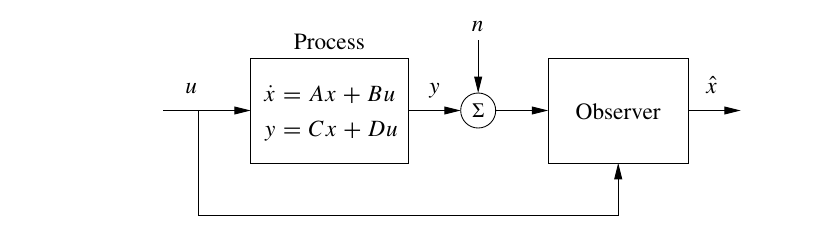
\includegraphics[scale=0.380]{img/output_feedback/observer_block_diagram.jpeg}
\end{center}
\caption{Block diagram for an observer. The observer uses the process measurement $y$
(possibly corrupted by noise $n$) and the input $u$ to estimate the current state of the process,
denoted $\hat{x}$.}
\label{observer_block_diagram}
\end{figure}


The problem of observability is one that has many important applications, even
outside feedback systems. If a system is observable, then there are no hidden dynamics inside it; we can understand everything that is going on through observation (over time) of the inputs and outputs. As we shall see, the problem of observability is of significant practical interest because it will determine if a set of sensors is
sufficient for controlling a system. Sensors combined with a mathematical model
can also be viewed as a virtual sensor that gives information about variables that
are not measured directly. The process of reconciling signals from many sensors
with mathematical models is also called sensor fusion.



\section{Testing for Observability}
\label{test_observability}

When discussing reachability in the last chapter, we neglected the output and focused on the state. Similarly, it is convenient here to initially neglect the input and
focus on the autonomous system



\begin{framed}
\theoremstyle{remark}
\begin{remark}{\textbf{Autonomous System}}

\end{remark}
\end{framed}

\begin{equation}
\frac{dx}{dt} = Ax ~~ y = Cx
\end{equation}

The objective is to understand when it is possible to determine the state from observations of the output. From

\begin{equation}
y = Cx
\end{equation}

we see that the output itself gives us the projection of the state $x$ on vectors that are rows of the matrix $C$. The 
observability problem can  immediately be solved if the matrix $C$ is invertible. If the matrix is not invertible we can take the derivatives and obtain

 
\begin{equation}
\frac{dy}{dt} = C\frac{dx}{dt} = CAx
\end{equation}

From the derivative of the output we thus get the projection of the state on vectors that are rows of the matrix $CA$. Proceeding in this way, we get

\begin{equation}
\begin{bmatrix}
 y \\
 y^{(1)} \\
 \vdots \\
 y^{(n-1)} 
\end{bmatrix} = 
\begin{bmatrix}
 C \\
 CA \\
 \vdots \\
 CA^{n-1} 
\end{bmatrix}x
\end{equation}

We thus find that the state can  be  determined if the observability matrix
 
\begin{equation}
W_o= 
\begin{bmatrix}
 C \\
 CA \\
 \vdots \\
 CA^{n-1} 
\end{bmatrix}
\end{equation}

has $n$ independent rows.  It turns out  that  we  need  not consider any derivatives higher
than $n-1$ (this is an application of the Cayley-Hamilton theorem)
 
\begin{framed}
\theoremstyle{remark}
\begin{remark}{\textbf{System with inputs}}

The calculation can easily be extended to systems with inputs. The state is then
given by a linear combination of inputs and outputs and their higher derivatives.
The observability criterion is unchanged. 
\end{remark}
\end{framed}


\begin{framed}
\theoremstyle{theorem}
\begin{theorem}{\textbf{Observability rank condition}}

A linear system of the form  
\begin{equation}
\frac{dx}{dt} = Ax + Bu, ~~ y = Cx + Du \nonumber
\end{equation}

is observable if and only if the observability matrix $W_o$ is full rank.
\end{theorem}
\end{framed}

\section{Observable Canonical Form}
\label{observability_canonical_form}

As in the case of reachability, certain canonical forms will be useful in studying ob-
servability. A linear single-input, single-output state space system is in observable
canonical form if its dynamics are given by


\begin{framed}
\theoremstyle{remark}
\begin{remark}{\textbf{Observable Canonical Form for Nonlinear Systems}}

The definition can be extended to systems with many inputs; the only difference is
that the vector multiplying u is replaced by a matrix.
\end{remark}
\end{framed}


The characteristic polynomial for a system in observable canonical form is

\begin{equation}
\lambda(s) = s^n +\alpha_1s^{n-1} + \ldots + \alpha_{n-1}s + \alpha_n
\end{equation}

In order to check the observability property of a systme more formally, we can compute the observability matrix for
a system in observable canonical form. This is given by

\begin{equation}
W_o= 
\begin{bmatrix}
 1 & 0 & 0 & \ldots &  0\\
 -\alpha_1 & 1 & 0 & \ldots &  0 \\
 -\alpha_{1}^{2} - \alpha_1 \alpha_2 & - \alpha_1 & 1 &  \ldots &  0 \\
 \vdots & \vdots & \vdots & \ddots & \vdots \\
* & * & * & \ldots & 1
\end{bmatrix} 
\end{equation}


where * represents  an entry  whose exact  value  is  not important.
What is important here is the rows of this matrix are linearly independent (since it is lower triangular), and hence Wo is full rank. Hence, it is invertible. 

As in the case of reachability (see section \ref{reachable_canonical_form}), it  turns  out  that  if a  system  is  observable then there
always exists a transformation $T$ that converts the system into observable canonical
form. This is useful for proofs since it lets us assume that a system is in observable
canonical form without any loss of generality. The observable canonical form may
be poorly conditioned numerically.
 

\section{State Estimation}
State feedback control design, as explained in t chapter \ref{state_feedback} requires that we have access to the complete state vector. 
However, measuring the complete state vector is not always feasible (for example a sensor may not be available at all) and it may also be expensive.
In this section we will introduce the idea of state estimation as a way to get access to the state variables. 


\begin{framed}
\theoremstyle{remark}
\begin{remark}{\textbf{Soft Sensors}}


The concept of using software instead of sensors to access the quantity we are 
interested in, is referred to as soft sensors in the automotive industry.
\end{remark}
\end{framed}

Recall that the idea of state feedback control was to modify the eigenvalues of the system under consideration by using the input

\begin{equation}
u = -Kx + K_r r  
\end{equation}

However, it can be seen that this requires the state vector $x$. The idea of state estimation is to design something called an observer that tries to provide an 
estimate say $\hat{x}$ of the state vector $x$. The observer is fed with the same input as the real plant. The goal of the observer is to provide somehow a replica of the true state vector.
Thus, we would like to have the error $\tilde{x}$ between the two quantities to be zero. Namely,


\begin{equation}
\tilde{x} = x - \hat{x} = 0 
\end{equation}
 
In this section, we want to construct a dynamical system of the form

\begin{equation}
\frac{d \hat{x}}{dt} = F\hat{x} + Gu + Hy  
\end{equation}

where $u$ and $y$ are the input and output of the original system and $\hat{x} \in R^n$ is an estimate of $x$ with the property

\begin{equation}
\hat{x}(t) \rightarrow x(t), ~~ \text{as} ~~ t \rightarrow \infty  
\end{equation}

Let's consider again the system

\begin{equation}
\frac{dx}{dt} = Ax + Bu ~~ y = Cx + Du
\label{sys}
\end{equation}

assume further that $D$ is zero. Assuming that the input $u$ is known, then an estimate of the state $x$ is given by

\begin{equation}
\frac{d\hat{x}}{dt} = A\hat{x} + Bu
\label{observer_one} 
\end{equation}  

We would like to know the properties of this estimate; how far is from the exact state? The estimation error is \cite{Astrom} 

\begin{equation}
\tilde{x} = x - \hat{x} 
\end{equation} 

substituting into equation \ref{observer_one} we find that


\begin{equation}
\frac{d\tilde{x}}{dt} = A\tilde{x}  
\end{equation}  

We already know that the behavior of this system depends on the eigenvalues of $A$. Concretely, if matrix $A$ has all its eigenvalues in the left half-plane, the error $\tilde{x}$ will go to zero,
and hence equation \ref{observer_one} is a dynamical system whose output converges to the state
of the system \ref{sys}.


The observer given by equation \ref{observer_one} uses only the process input $u$; the measured
signal does not appear in the equation. We must also require that the system be stable,
and essentially our estimator converges because the state of both the observer and
the estimator are going zero. This is not very useful in a control design context since
we want to have our estimate converge quickly to a nonzero state so that we can
make use of it in our controller. We will therefore attempt to modify the observer
so that the output is used and its convergence properties can be designed to be fast
relative to the system’s dynamics. This version will also work for unstable systems.

Let's now consider the following observer

\begin{equation}
\frac{d \hat{x}}{dt} = A\hat{x} + Bu + L(y- C \hat{x})
\label{observer_two}   
\end{equation}

The term $L(y- C \hat{x})$ provides feedback and hence the observer in \ref{observer_two} can be seen as a generalization of the observer in \ref{observer_one}. The supplied feedback is proportional to the difference between the observed output and the output predicted by the observer. Substituting the expression for the error $\tilde{x}$ we arraive at

 \begin{equation}
\frac{d\tilde{x}}{dt} = (A-LC)\tilde{x} 
\label{observer_two}   
\end{equation} 

If the matrix $L$ can be chosen in such a way that the matrix $A-LC$ has eigenvalues with negative real parts, the error $\tilde{x}$ will go to zero. The convergence rate is determined by an appropriate selection of the eigenvalues.
 

\begin{framed}
\theoremstyle{remark}
\begin{remark}{\textbf{Observer design and state feedback duality}}


Notice the similarity between the problems of finding a state feedback and
finding the observer. State feedback design by eigenvalue assignment is equivalent
to finding a matrix $K$ so that $A-BK$ has given eigenvalues. Designing an observer
with prescribed eigenvalues is equivalent to finding a matrix $L$ so that $A-LC$ has
given eigenvalues. Since the eigenvalues of a matrix and its transpose are the same
we can establish the following equivalences:

\begin{equation}
A \leftrightarrow A^T, ~~ B \leftrightarrow C^T, ~~ K \leftrightarrow L^T, ~~ W_r \leftrightarrow W_{o}^{T}
\end{equation}

The observer design problem is the dual of the state feedback design problem. 
\end{remark}
\end{framed}



\begin{framed}
\theoremstyle{theorem}
\begin{theorem}{\textbf{Observer design by eigenvalue assignment}}


Consider the system

\begin{equation}
\frac{dx}{dt} = Ax + Bu, ~~ y =Cx   \nonumber
\end{equation} 

with one input and one output. Let the characteristic polynomial related to matrix A be

\begin{equation}
\lambda(s) = s^n + \alpha_1 s^{n-1} + \ldots + \alpha_{n-1}s + \alpha_n \nonumber
\end{equation}

If the systme is observable, then the dynamical system

\begin{equation}
\frac{d \hat{x}}{dt} = A\hat{x} + Bu + L(y- C \hat{x})  \nonumber
\end{equation}


is an observer for the system with $L$ chosen as 

\begin{equation}
L = W_{o}^{-1}\tilde{W}_o
\begin{bmatrix}
 p_1 - \alpha_1 \\
 p_2 - \alpha_2 \\
 \vdots  \\
 p_n - \alpha_n
\end{bmatrix} \nonumber
\end{equation}

The matrices $W_{o}$ and $\tilde{W}_{o}$ are given by

The resulting observer error $\tilde{x}$ is governed by a differential equation that has the following characteristic polynomial

\begin{equation}
p(s) = s^n +  p-1 s^{n-1} + \ldots + p_n  \nonumber
\end{equation}
\end{theorem}
\end{framed}

The dynamical system (7.10) is called an observer for (the states of) the system (7.9) because it will generate an approximation of the states of the system from its inputs and outputs. This form of an observer is a much more useful form than the one given by pure differentiation in equation (7.3).


\section{Questions}

\textbf{Question 1}

What is the main reason for using an estimator in feedback control?

\begin{itemize}
\item A) There are process disturbances in the model 
\item B) We are measuring the wrong quantities 
\item C) It is too expensive or impractical to measure each state variable correct 
\end{itemize} 

\textbf{Answer}  

Option C is the correct answer.


%\chapter{Kalman Filters}
\label{kalman_filters}

Kalman filtering is an iterative process that uses a set of equations and consecutive data inputs to quickly estimat the 
true value; e.g. position, velocity etc., of the object being measured when the measured values contain unpredicted or 
random error, uncertainty or variation.

One of the principal uses of observers in practice is to estimate the state of a
system in the presence of noisy measurements. We have not yet treated noise in our
analysis, and a full treatment of stochastic dynamical systems is beyond the scope
of this text. In this section, we present a brief introduction to the use of stochastic
systems analysis for constructing observers. We work primarily in discrete time to
avoid some of the complications associated with continuous-time random processes
and to keep the mathematical prerequisites to a minimum. This section assumes
basic knowledge of random variables and stochastic processes; see Kumar and
Varaiya [KV86] or Åström [Åst06] for the required material.

Consider again the LTI state-space model

\begin{equation}
\frac{dx}{dt} = Ax + Bu +v  ~~ y = Cx + Du +w 
\end{equation}
the model is augmented with additional terms representing the error or disturbance. Concretely,
$v$ is the process disturbance and $w$ is measurements noise. Both are assumed to be normally distibuted with zero mean;

\begin{eqnarray}
E[v] = 0, ~~ E[vv^T] = R_v, ~~ E[w] = 0, ~~ E[ww^T] = R_w 
\label{noise_proccess_1} 
\end{eqnarray}



\begin{framed}
\theoremstyle{remark}
\begin{remark}{\textbf{Normally distributed random variable}}

A one dimensional random variable $X$ is said to follow the normal distribution
\end{remark}
\end{framed}


\begin{framed}
\theoremstyle{remark}
\begin{remark}{\textbf{Nonlinear Systems}}

The definition above holds for nonlinear systems as well, and the results discussed here have extensions to the nonlinear case.
\end{remark}
\end{framed}

$R_v$ and $R_w$ are the covariance matrices for the process disturbance $v$ and the measurement noise $w$ respectively. Furthermore, we assume that the variables $v, w$ are not correlated i.e 

\begin{eqnarray}
E[vw^T] = 0
\label{noise_proccess_2} 
\end{eqnarray}


\begin{framed}
\theoremstyle{remark}
\begin{remark}{\textbf{Corralated random variables}}

Two random variables $X$ and $Y$ are said to be linearly correlated 
\end{remark}
\end{framed}

The initial condition is also modeled as a Gaussian random variable

\begin{eqnarray}
E[x(0)] = x_0, ~~ E[x(0)x^{T}(0)] = P_0
\label{noise_proccess_3} 
\end{eqnarray}

Implementation of the state-space model in a computer requires discretization. Thus the system can be written as discrete-time linear system with dynamics governed by

\begin{equation}
x_{t+1} = Ax_t + Bu_t + Fv_t,  ~~ y_t = Cx_t + w_t 
\end{equation}

Given the measurements $\{y(\tau), 0 \leq \tau \leq t \}$, we would like to find an estimate $\hat{x}_t$ that minimizes the mean square error:

\begin{equation}
E[(x_t - \hat{x}_t)(x_t - \hat{x}_t)^T] 
\end{equation}

\begin{framed}
\theoremstyle{theorem}
\begin{theorem}{\textbf{Kalman 1961}}


Consider the random process $x_t$ with dynamics described by  

\begin{equation}
x_{t+1} = Ax_t + Bu_t + Fv_t,  ~~ y_t = Cx_t + w_t \nonumber
\end{equation} 

and noise processes and initial conditions described by \ref{noise_proccess_1},  \ref{noise_proccess_2} and 
\ref{noise_proccess_3}. The observer gain $L$ that minimizes the mean square error is given by  

\begin{equation}
L_t = AP_tC^T(R_w + CP_tC^T)^{-1}  \nonumber
\end{equation}

where

\begin{equation}
P_{t+1} =  (A − LC)P_t(A − LC)^T + R_v LR_w L^T, ~~ P_0 = E[x_0x^{T}_0\}
\end{equation}

\end{theorem}
\end{framed}

A proof of this result can be found in \cite{Astrom}. We, note, however the following points:

\begin{itemize}
\item the Kalman filter has the form of a recursive filter: given mean square error $P_t$ at time $t$, we can compute how the estimate and error change. Thus we do not need to keep track of old values of the output.
\item Furthermore, the Kalman filter gives the estimate $\hat{x}_t$ and the error covariance $P_t$, so we can see how reliable the estimate is. 
It can also be shown that the Kalman filter extracts the maximum possible information about output data. 
If we form the residual between the measured output and the estimated output,
\end{itemize}

\begin{equation}
e_t = y_t - C\hat{x}_t
\end{equation}
we can show that for the Kalman filter the error covariance matrix $R_e$ is

\begin{equation}
R_e(i,j) = E(e_{j}e_{k}^{T}) = W_t\delta_{jk} 
\end{equation}

In other words, the error is a white noise process, so there is no remaining dynamic information content in the error.




\begin{framed}
\theoremstyle{theorem}
\begin{theorem}{\textbf{Kalman-Bucy 1961}}


The optimal estimator has the form of a linear observer 

\begin{equation}
\frac{d\hat{x}}{t} = A\hat{x} + Bu + L(y - C\hat{x}),  ~~ \hat{x}(0) = E(x(0)) \nonumber
\end{equation} 

where $L$ is given by

\begin{equation}
L = PC^TR_{w}^{-1}  \nonumber
\end{equation}

where $P$


\end{theorem}
\end{framed}


All matrices $A, B, C, R_v, R_w, P$ and $L$ can be time varying. The essential condition is that the Riccati equation (8.30) has a unique positive 
solution.

\section{Kalman’s Decomposition of a Linear System}

In this chapter and the previous one we have seen that two fundamental properties
of a linear input/output system are reachability and observability. It turns out that
these two properties can be used to classify the dynamics of a system. The key
result is Kalman’s decomposition theorem, which says that a linear system can be
divided into four subsystems:

\begin{itemize}
\item $\Sigma_{ro}$ which is reachable and observable
\item $\Sigma_{r\bar{o}}$ which is reachable but no observable 
\item $\Sigma_{\bar{r}o}$ which is not reachable but is observable
\item $\Sigma_{\bar{r}\bar{o}}$which is neither reachable nor observable
\end{itemize}


Thus from the input/output point of view, it is only the reachable and observable
dynamics that matter.


\begin{framed}
\theoremstyle{remark}
\begin{remark}{\textbf{Kalman's decomposition for state-space}}

The general case of the Kalman decomposition is more complica
ted and requires some additional linear algebra; see the original pap
er by Kalman, Ho, and Narendra [KHN63]. The key result is that the state space can still be decomposed
into four parts, but there will be additional coupling so that the equations have the form 
\end{remark}
\end{framed}





%\begin{appendices}
% \input{appendices/install_python/install_python_linux.tex}
% \input{appendices/install_python/install_python_win.tex}
%\input{appendices/source_code_for_vector_addition.tex}

%\end{appendices}

\clearpage

\bibliographystyle{plain}
\input{references.bbl}
\bibliography{JabRef.bib}


\end{document}
